\documentclass[12pt]{scrartcl}
\usepackage{graphicx}
\usepackage[default]{opensans}
\usepackage{sfmath} % sans font also for math
 \usepackage[binary-units = true]{siunitx}

% defining the paper layout that no text overlaps with the header
\usepackage[
  top=35mm,
  headheight=25mm,
  headsep=3mm,
  bottom=30mm,
  left=25mm,
  right=25mm
]{geometry}

\usepackage{latexsym}
\usepackage[centertags]{amsmath}
\usepackage{amssymb}

% custom header and footpage
\usepackage{scrpage2}
\pagestyle{scrheadings} % you have to set the custom layout
% Head
\ihead{M4.2} % left head
%\chead{}
\ohead{
\includegraphics[height=25mm]{figures/EUCALL.png}}
% Foot
\ifoot{
\includegraphics[height=13.4mm]{figures/EU.png}} % left foot
\cfoot{%
  \begin{minipage}{100mm}%
    \begin{scriptsize}%
      \normalfont{This project has received funding from the}
      \textit{European Union’s Horizon 2020 research and innovation programme}
      \normalfont{under grant agreement No 654220.}
    \end{scriptsize}%
  \end{minipage}%
} % center foot
\ofoot{\thepage} % right foot

\usepackage{booktabs}

%%%%%%%%%%%%%%%%%%%%%%%%%%%%%%%%%%%%%%%%%%%%%%%
%   BIBLIOGRAPHY SETTINGS                     %
%%%%%%%%%%%%%%%%%%%%%%%%%%%%%%%%%%%%%%%%%%%%%%%
\usepackage[bibstyle=nature,sorting=none,=maxnames=1000,eprint=false,
defernumbers=true, backend=biber]{biblatex}
\usepackage{hyperref}

\renewcommand*\finalnamedelim{, and\addspace}
\DeclareNameAlias{sortname}{last-first}
\renewcommand{\newunitpunct}{, }

\AtEveryBibitem{%
  \clearfield{day}%
  \clearfield{month}%
  \clearfield{endday}%
  \clearfield{endmonth}%
  \clearfield{issn}%
  \clearfield{issue}%
}
%convert titles to hyperlinks using doi
\ExecuteBibliographyOptions{doi=false} \newbibmacro{string+doi}[1]{%
  \iffieldundef{doi}{#1}{\href{http://dx.doi.org/\thefield{doi}}{#1}}}
  \DeclareFieldFormat*{title}{\usebibmacro{string+doi}{\mkbibemph{#1}}}

\addbibresource{aux.bib}
\addbibresource{references.bib}
%%%%%%%%%%%%%%%%%%%%%%%%%%%%%%%%%%%%%%%%%%%%%%%
% END BIBLIOGRAPHY SETTINGS                   %
%%%%%%%%%%%%%%%%%%%%%%%%%%%%%%%%%%%%%%%%%%%%%%%


% sophisticated linking of references in the pdf and setting some options
\usepackage{url}                                                  % for correct typesettings of URLs
\usepackage{hyperref}                                             % for sophisticated linking of urls, dois, pictures, tables, etc.
\hypersetup{
    unicode=true,                                                 % non-Latin characters in Acrobat’s bookmarks
    pdftoolbar=true,                                              % show Acrobat’s toolbar?
    pdfmenubar=true,                                              % show Acrobat’s menu?
    pdffitwindow=false,                                           % window fit to page when opened
    pdftitle={M4.2: First example simulation},                    % title
    pdfauthor={C. Fortmann-Grote},                                % author
    pdfsubject={EUCALL WP4 (SIMEX) Milestone 4.2},                % subject of the document
    pdfcreator={pdflatex},                                        % creator of the document
    pdfkeywords={EUCALL, SIMEX, simulations},                     % list of keywords
    pdfnewwindow=true,                                           % links in new PDF window
    colorlinks=true,                                             % false: boxed links; true: colored links
    linkcolor=blue,                                              % color of internal links (change box color with linkbordercolor)
    citecolor=blue,                                              % color of links to bibliography
    filecolor=blue,                                              % color of file links
    urlcolor=blue                                                % color of external links
}

% Zeilenabstand
\renewcommand{\baselinestretch}{1.2}


%%%%%%%%%%%%%%%%%%%%%%%%%%%%%%%%%%%%%%%%%%%%%%%
% END BIBLIOGRAPHY SETTINGS                   %
%%%%%%%%%%%%%%%%%%%%%%%%%%%%%%%%%%%%%%%%%%%%%%%

\begin{document}
\makeatletter
\begin{titlepage}
\thispagestyle{scrheadings}
\begin{center}
  $~$\\
  \vspace{2cm}
  \Huge{\textbf{WP 4 -- SIMEX\\[1cm]
    Milestone M4.2: Demonstration of a first example simulation%
  }}\\
  \vspace{2cm}
  \large{ Carsten Fortmann-Grote}
  \vspace{1cm}
  \date{\today}
\end{center}
\vfill%
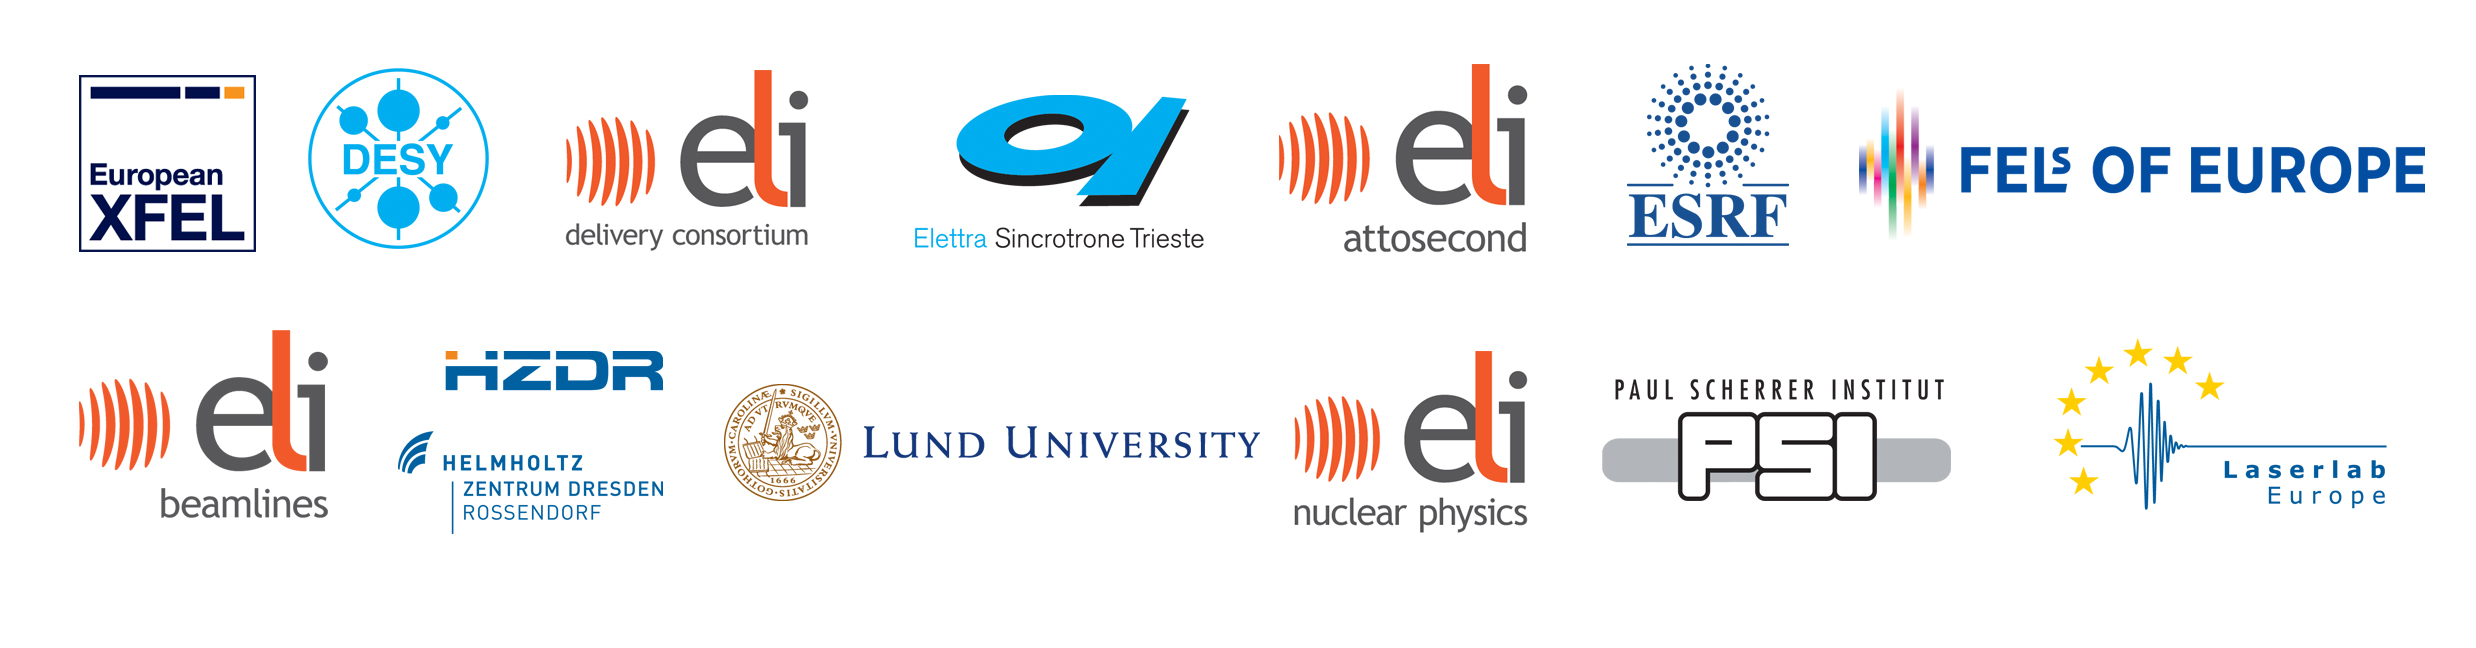
\includegraphics[width=\textwidth]{figures/PartnerLogos_2017}
\normalfont
\end{titlepage}
\makeatother
%
\tableofcontents
%
\section{Summary}
Milestone M4.2 (as detailed in Task 4.2.1) of the SIMEX workpackage in EUCALL is the demonstration of a
first example simulation. In this example, we simulate a single--particle
imaging experiment at the European X--ray Free Electron Laser. FEL pulses of
\SIlist{3;9;30}{\fs} pulse duration and \SI{4.96}{\keV} photon energy are propagated
through the SASE 1 beamline and the focusing optics of the SPB-SFX scientific
instrument. In the focus, the photons interact with the 2NIP molecule and
scatter into a pixel area detector situated \SI{13}{cm} behind the sample. We
save each simulated diffraction pattern and feed the patterns into the
orientation reconstruction algorithm EMC. Statistical analysis of oriented 3D
diffraction datasets allows to assess the data quality of our simulated data as
a function of the pulse duration, which is is controlled through the machine
parameters of the FEL, in particular the electron bunch charge.

The results of this study analyis of the simulated diffraction patterns are published in
Ref.~\cite{Fortmann-Grote2017}. In addition, we published the individual
datasets resulting from the simulations on the
\href{https://zenodo.org/communities/eucall-data}{EUCALL Data Repository} hosted
on \href{https://www.zenodo.org/}{Zenodo}. We note in passing that the
deposition of diffraction data from a non--plasma sample~\cite{Fortmann-Grote2017.zenodo.886087}
partially fulfills SIMEX Deliverable D4.4. Coherent diffraction data
from a plasma sample was accomplished in Milestone M4.3 (Interoperability of
simulations)~\cite{EUCALL_SIMEX_M4.3}.

Tutorials for the individual simulation steps can be found on the
\href{https://www.github.com/eucall-software/simex_platform/wiki/SimEx-Tutorial}{SIMEX wiki} and
on the
\href{https://www.youtube.com/channel/UC5H8cATZiUPNfF7P_xEhBpQ/videos}{EUCALL youtube channel}.
Finally, the \href{https://eucall-software.github.io/simex_platform/}{reference manual} of the simulation environment simex\_platform
contains a description of the data formats of all relevant simulation datasets, see also
Milestone M4.1~\cite{EUCALL_SIMEX_M4.1}.

Newer simulations, studying proteins embedded in
a solvent (water) were recently presented at the Optics and Photonics Conference
2017~\cite{Fortmann-Grote2017b}.

\section{Supporting material}
\begin{tabular}[ht]{|r|r|r|r|}
  \hline
  \textbf{Module}       & \textbf{Dataset}  &
  \textbf{Usage instruction}   & \textbf{Data format}       \\
  \hline
    FEL source &
    \href{https://dx.doi.org/10.5281/zenodo.855301}{10.5281/zenodo.855301} &
    \href{https://github.com/eucall-software/simex_platform/wiki/SimEx-Tutorial#prepating-the-source-input}{Manual}
    \href{https://youtu.be/Ql1p5-CLHug}{Video} &
    \href{https://eucall-software.github.io/simex_platform/#fel-source-calculations-fast}{Manual}
  \\
    Propagation &
    \href{https://dx.doi.org/10.5281/zenodo.884873}{10.5281/zenodo.884873} &
    \href{https://github.com/eucall-software/simex_platform/wiki/SimEx-Tutorial#beamline-propagation}{Manual} &
    \href{https://eucall-software.github.io/simex_platform/#coherent-wavefront-propagation-wpg-srw}{Manual}
  \\
    Interaction &
    \href{https://dx.doi.org/10.5281/zenodo.886061}{10.5281/zenodo.886061} &
    \href{https://github.com/eucall-software/simex_platform/wiki/SimEx-Tutorial#photon-matter-interaction}{Manual} &
    \href{https://eucall-software.github.io/simex_platform/#photon-matter-interaction-xmdyn}{Manual}
  \\
    Diffraction &
    \href{https://dx.doi.org/10.5281/zenodo.886087}{10.5281/zenodo.886087} &
    \href{https://github.com/eucall-software/simex_platform/wiki/SimEx-Tutorial#diffraction}{Manual} &
    \href{https://eucall-software.github.io/simex_platform/#diffraction-singfel}{Manual}
  \\
  \hline
\end{tabular}
%

\printbibliography[notkeyword=zenodo,notkeyword=eucall, notkeyword=simex, notkeyword=tutorial, title={Articles}]
\printbibliography[notkeyword=zenodo,notkeyword=tutorial, keyword=simex, keyword=eucall, title={EUCALL Reports}]
\printbibliography[keyword=zenodo,notkeyword=tutorial, title={Datasets}]
%
%\nocite{Fortmann-Grote_Zenodo855301}
%\printbibliography[keyword=zenodo, title={Datasets}]
%
%\nocite{Fortmann-Grote_Youtube_XPD}
%\printbibliography[keyword=tutorial, title={Tutorials}]


\end{document}


